\documentclass{beamer}
\usepackage[utf8]{inputenc}   % pour pouvoir taper les accents directement     
\usepackage{amsfonts,amssymb,amsmath}
\usepackage{tikz}
\usepackage{array}
\usepackage{calc}
\usetikzlibrary{patterns}
\usepackage[absolute,showboxes,overlay]{textpos}     
\textblockorigin{0pt}{0pt}                          
\TPshowboxesfalse  
 \usepackage{lmodern,multido}

\newcommand{\R}{\mathbb{R}}
\newcommand{\C}{\mathbb{C}}
\newcommand{\Z}{\mathbb{Z}}
\newcommand{\N}{\mathbb{N}}
\newcommand{\Q}{\mathbb{Q}}

\begin{document}
 %%%%%%%%%%%%%%%%%%%%%%%%%%%%%%%%%%%%%%%%%%%%%%%%%%%%%%%%%%%%%%%
 % Afficher le numéro de diapos 
  \addtobeamertemplate{navigation symbols}{}{ \hspace{1em}    \usebeamerfont{footline}%
    \insertframenumber/\inserttotalframenumber }
 %%%%%%%%%%%%%%%%%%%%%%%%%%%%%%%%%%%%%%%%%%%%%%%%%%%%%%%%%%%%%%%

\begin{frame}{Introduction aux statistiques}


\begin{center}{\bf \Large Chapitre 2} \end{center}
\begin{center}{\bf \Large Lois des grands nombres et approximations} \end{center}
\vspace{0.3cm}
\begin{itemize}
\item Lois des grands nombres
\item Théorème Centrale Limite
\item Loi Binomiale et loi Normale
\item Loi de Poisson et loi Normale
\end{itemize}


\end{frame} 

 %%%%%%%%%%%%%%%%%%%%%%%%%%%%%%%%%%%%%%%%%%%%%%%%%%%%%%%%%%%%%%%

\begin{frame}{Loi des grands nombres}
%\begin{textblock*}{\textwidth}(1cm,2cm)

%Si 
\begin{itemize}
\item  $X_1, X_2, \ldots, X_n, \ldots$ iid %indépendantes  et identiquement distribuées 
de moyenne (théorique) $\mu$ ;
\item Si $M_n=\frac{1}{n}\sum\limits_{i=1}^{n} X_i$ (moyenne empirique) ;
\item alors $M_n \to \mu$ lorsque $n\to\infty$ (convergence lente).
\end{itemize}
\begin{center}
  \textcolor{red}{Si $n$ est grand}, $M_n$ est un bon estimateur de $\mu$. \\
  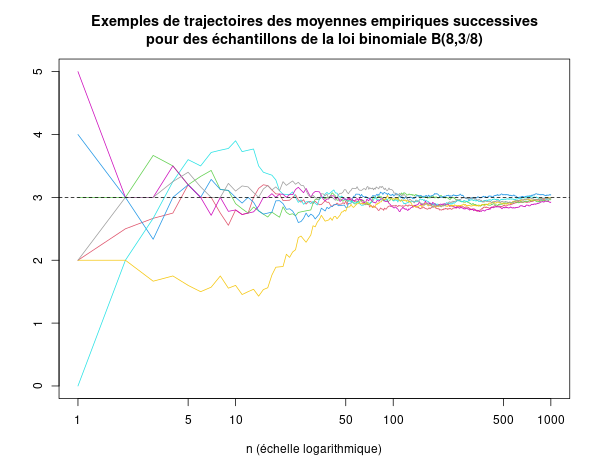
\includegraphics[width=0.5\textwidth]{images/Rplot_trajectoires_moyenne_empirique.png}
\end{center}
%\end{textblock*}
\end{frame}
 
 
% \begin{frame}{Approximations de lois}
% \begin{textblock*}{\textwidth}(1cm,2cm)
% 
% \begin{center}{\bf \Large Loi des grands nombres} \end{center}
% Si 
% \begin{itemize}
% \item  $X_1, X_2, ..., X_n,$ indépendantes  et identiquement distribuées de moyenne
% $\mu$ et d'écart-type $\sigma$ ;
% \item $M_n=\frac{1}{n}\sum\limits_{i=1}^{n} X_i$ ;
% \end{itemize}
% \begin{minipage}{0.5 \textwidth}
% alors \textcolor{red}{ si $n$ est grand}
%  \begin{itemize}
% \item $M_n \approx \mathcal{N}(\mu,\frac{\sigma}{\sqrt{n}})$
% soit  $\frac{M_n-\mu}{\sigma/\sqrt{n}} \approx \mathcal{N}(0,1)$
% \end{itemize}
% 
% \
% 
% Remarque : convergence lente 
% \end{minipage}
% \begin{minipage}{0.4 \textwidth}
% \begin{center}
% 
% \begin{tikzpicture}[xscale=1.7,yscale=0.3]
% \draw (0,-1) node {$0$};
% \draw (1,-1) node {$1$};
% \draw[->] (-0.5,0) -- (1.5,0);
% \draw[->] (0,-0.5) -- (0,7);
% %\foreach \k in {1,10}
% %{
% %\only<\k>
% %{
% %\draw plot file {data/densite_grands_nombres_\k.txt} ;
% %\draw[red,dashed] plot file {data/densite_grands_nombres_norm_\k.txt} ;
% %\draw (1.2,6.5) node {$n=\k$} ;
% %}
% %}
% 
% \only<1>
%  {
% \draw plot file {data/densite_grands_nombres_1.txt} ;
% \draw[red,dashed] plot file {data/densite_grands_nombres_norm_1.txt} ;
% \draw (1.2,6.5) node {$n=1$} ;
% }
% 
% \only<2>
%  {
% \draw plot file {data/densite_grands_nombres_10.txt} ;
% \draw[red,dashed] plot file {data/densite_grands_nombres_norm_10.txt} ;
% \draw (1.2,6.5) node {$n=10$} ;
% }
% 
% \end{tikzpicture}
% \end{center}
% \end{minipage}
% 
%  \end{textblock*}
% 
% \end{frame}

 %%%%%%%%%%%%%%%%%%%%%%%%%%%%%%%%%%%%%%%%%%%%%%%%%%%%%%%%%%%%%%%

%\begin{frame}{Approximations de lois}
\begin{frame}{Théorème Central Limite}

% \begin{center}{\bf \Large Théorème Central Limite} \end{center}
Si $X_1, X_2, ..., X_n$ 
\begin{itemize}
\item indépendantes ;
\item de lois de probabilités quelconques ;
\item  d'espérance $E(X_i)$ et de variance finie $\sigma_i^2$ ;
\end{itemize}

et si 
\begin{itemize}
\item $M_n=\sum\limits_{i=1}^n X_i$
\end{itemize}
alors pour $n$ grand ($n\geq 30$), $M_n$ suit approximativement
une loi normale $\mathcal{N}(\mu,\sigma)$ avec $\mu = \sum\limits_{i=1}^n E(X_i)$ et
$\sigma = \sqrt{\sum\limits_{i=1}^n \sigma_i^2}$. 


\end{frame} 
 



 %%%%%%%%%%%%%%%%%%%%%%%%%%%%%%%%%%%%%%%%%%%%%%%%%%%%%%%%%%%%%%%

\begin{frame}{Approximations de lois}
%\begin{textblock*}{\textwidth}(1cm,2cm)

\begin{center}{\bf \large loi Binomiale et loi Normale } \end{center}

 \vspace{0.5cm}

\begin{minipage}{0.6\textwidth}
Si 
\begin{itemize}
\item $X\sim \mathcal{B}(n,p)$ 
\item $n$ grand : $n\geq 30$ 
\item $p$ moyen : $np\geq 5$ et  $n(1-p)\geq 5$ \\
\end{itemize} 
 \vspace{0.2cm}
alors $X$ suit approximativement une loi normale \small $\mathcal{N}(np, \sqrt{np(1-p)})$.
\end{minipage}
\begin{minipage}{0.15 \textwidth}
\begin{center}
\begin{tikzpicture}[xscale=0.2,yscale=3.8]
\draw[->] (-0.5,0) -- (23,0);
\draw[->] (0,-0.01) -- (0,1);

	\foreach \k in {0,1,...,30}
	{	
	    \draw[blue] plot file {data/approx_binom2_1_\k.txt} node {$\bullet$} ;
		\draw[red] plot file {data/approx_binom2_20_\k.txt} node {$\bullet$} ;
	}	
		\draw[blue] plot file {data/densite_approx_binom_norm_1.txt} node {$\times$} ;
		\draw[red] plot file {data/densite_approx_binom_norm_20.txt} node {$\times$} ;
\draw[blue] (4,0.8) node {$n=1$};	
\draw[red] (10,0.3) node {$n=30$};	

\end{tikzpicture}
\end{center}
\end{minipage}
 
 \vspace{0.5cm}
 
  {\bf Attention} : si $X$ discrète approximée  par $Y$ continue :

 \small $
Pr(X=k)=Pr(k-0,5 \leq X \leq k+0,5) \approx Pr( k-0,5 \leq Y \leq
k+0,5).
$

%\end{textblock*}

\end{frame} 

 %%%%%%%%%%%%%%%%%%%%%%%%%%%%%%%%%%%%%%%%%%%%%%%%%%%%%%%%%%%%%%%

\begin{frame}{Approximations de lois}
%\begin{textblock*}{\textwidth}(1cm,2cm)

\begin{center}{\bf \large Loi de Poisson et loi Normale } \end{center}

 \vspace{0.5cm}

\begin{minipage}{0.6\textwidth}
Si 
\begin{itemize}
\item $X\sim \mathcal{P}(\lambda)$ 
\item $\lambda >5$ 
\end{itemize}
 \vspace{0.2cm}
alors $X$ suit approximativement une loi normale $\mathcal{N}(\lambda,\sqrt{\lambda})$.
\end{minipage}
\begin{minipage}{0.15 \textwidth}
\begin{center}
\begin{tikzpicture}[xscale=0.2,yscale=5]
\draw[->] (-0.5,0) -- (23,0);
\draw[->] (0,-0.01) -- (0,0.6);

\only<1>
{
	\foreach \k in {0,1,...,20}
	{	
		\draw[black] plot file {data/approx_pois_1_\k.txt} node {$\bullet$ };
		\draw[green] plot file {data/approx_pois_10_\k.txt} node {$\bullet$ };
	}	
	\draw[black] plot file {data/densite_approx_poiss_norm_1.txt} ;
	\draw[green] plot file {data/densite_approx_poiss_norm_10.txt} ;
\draw[black] (3,0.5) node {$\lambda=1$} ;
\draw[green] (15,0.2) node {$\lambda=10$} ;
}

\end{tikzpicture}
\end{center}
\end{minipage}

 
 \vspace{0.5cm}
 
   {\bf Attention} : si $X$ discrète approximée  par $Y$ continue :

\small $
Pr(X=k)=Pr(k-0,5 \leq X \leq k+0,5) \approx Pr( k-0,5 \leq Y \leq
k+0,5).
$


%\end{textblock*}

\end{frame}  


%%%%%%%%%%%%%%%%%%%%%%%%%%%%%%%%%%%%%%%%%%%%%
\end{document}










 








